\documentclass[aspectratio=169]{beamer}
\usepackage{xcolor}
\usepackage{tikz}
\usepackage{graphicx}
\graphicspath{ {./src/img/} }

\usetheme{Boadilla}
\usecolortheme{rose}
% \beamerdefaultoverlayspecification{<+->} % this will turn it into slides

\title{NEXTGEN}
\subtitle{The \textit{Secret} Breakthrough Technology}
\author{George Onoufriou, Paul Mayfield, Georgios Leontidis}
\date{\today}

\begin{document}

  % \definecolor{TXT}{RGB}{238,238,238} % #EEEEEE
  % \definecolor{BG}{RGB}{68,68,68} % #444
  % %
  % \setbeamercolor{background canvas}{bg=BG}
  % \color{TXT}

  \begin{frame}
    \titlepage
    \begin{center}
      
\includegraphics[width=0.3\linewidth]{ioft.png}
    \end{center}
  \end{frame}

\addtobeamertemplate{frametitle}{}{%
\begin{tikzpicture}[remember picture,overlay]
\node[anchor=north east,yshift=2pt] at (current page.north east) {
\includegraphics[height=0.8cm]{ioft.png}};
\end{tikzpicture}}


  \section{Intro}

    \begin{frame}{Contents}
      \tableofcontents
    \end{frame}

    \begin{frame}{History}
      In last years 2019 IoFT Conference:
      \begin{itemize}
        \item Data and its importance to the agri-food industry.
        \item Problems were announced; data, data sharing, trust, sensitivity.
        \item Possible approaches proposed by others; data-trusts, block-chain, distributed ledgers.
        \item While these are good solutions to open participants, they lack privacy.
        \item We proposed alternative technical solution that is a first step in the chain of trust.
        \item We are here today, coming full circle, to present our research and solution.
        \item Without further ado, let me re-introduce ...
      \end{itemize}
      % 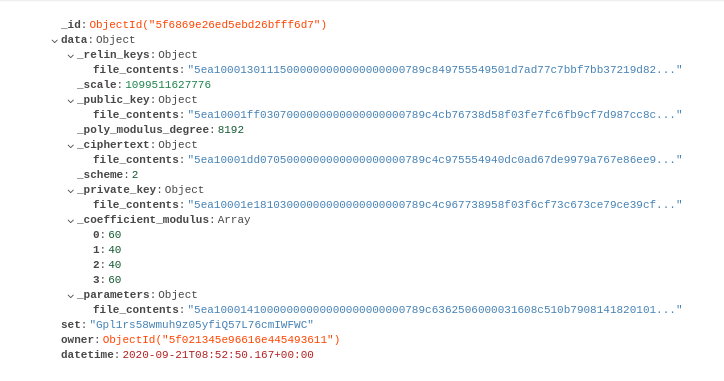
\includegraphics[width=0.5\linewidth]{data.png}
    \end{frame}

    \begin{frame}{Fully Homomorphic Encryption}
      \begin{columns}
        \begin{column}{0.5\textwidth}
          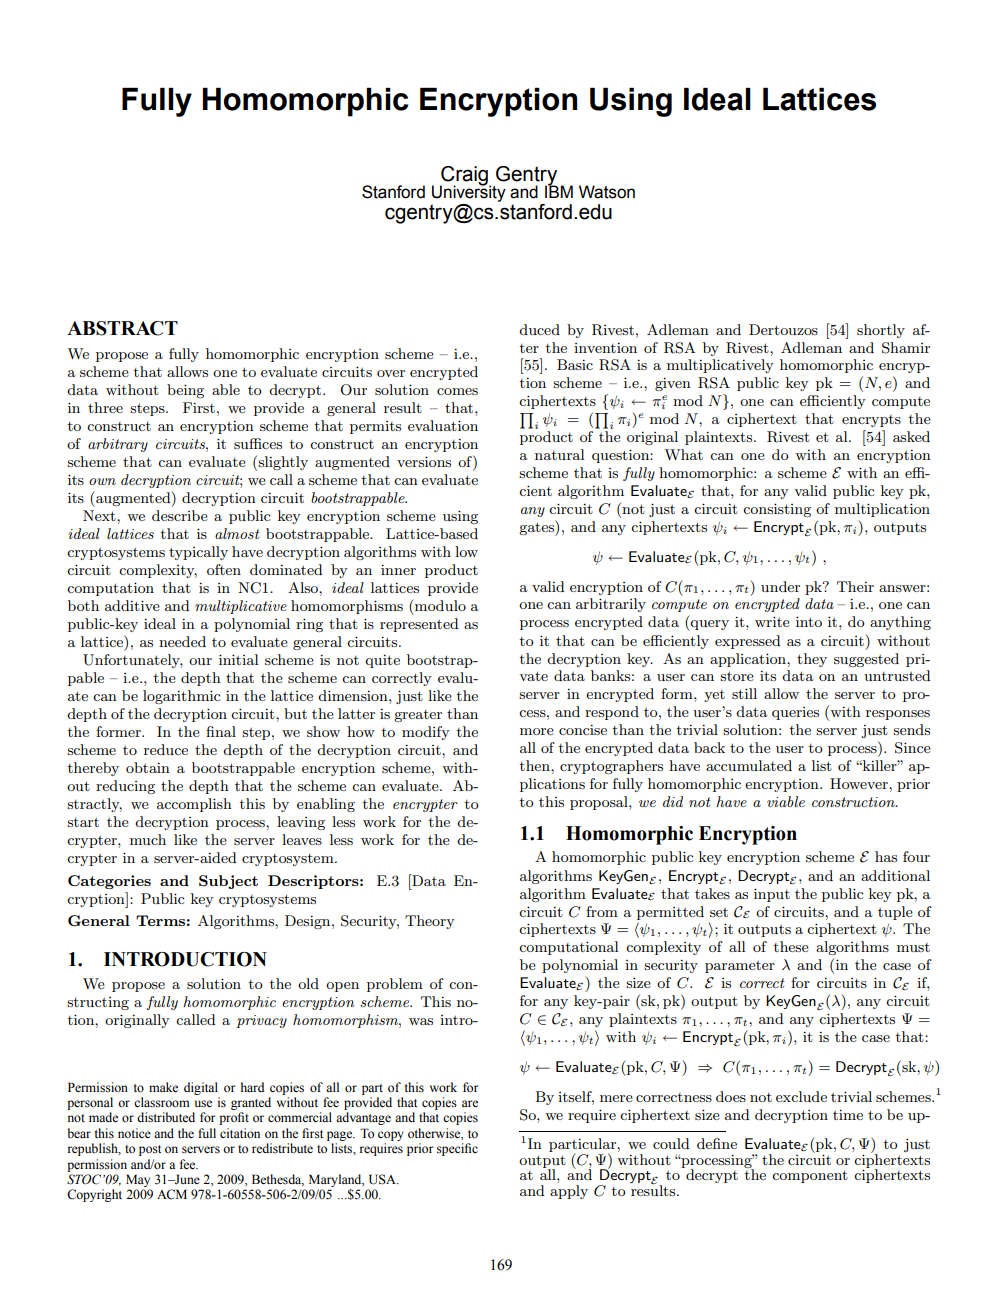
\includegraphics[width=0.75\linewidth]{gentry.png}
          \cite{gentry2009fully}
        \end{column}
        \begin{column}{0.5\textwidth}
          \begin{itemize}
            \item "Holy grail of encryption"
            \item Arbitrary computational depth on ciphertext
            \item Quantum decryption resistant ciphertext
            \item Abelian group operations \{+n,+(-n),*n\} on ciphertext
            \item Unable to compute non abelian operations such as division
          \end{itemize}
        \end{column}
      \end{columns}
    \end{frame}

    \begin{frame}{Deep Learning}
      \begin{columns}
        \begin{column}{0.5\textwidth}
          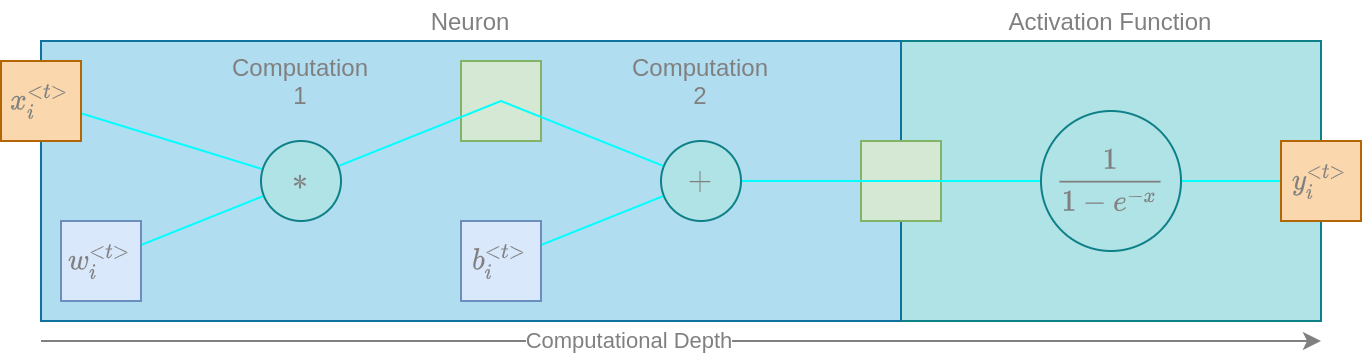
\includegraphics[width=1\linewidth]{neuron.png}
        \end{column}
        \begin{column}{0.5\textwidth}
          \begin{itemize}
            \item A subset of machine learning, which seeks to use neural networks to learn the distribution of data, without manual feature engineering.
            \item State-of-the-art in almost all machine learning tasks (Image recognition, Classification, sequence generation, etc)
            \item Usually a large computational depth, due to layers and layers of neurons and activation functions.
          \end{itemize}
        \end{column}
      \end{columns}
    \end{frame}

  \section{Methodology}

    \begin{frame}{Deep Learning $+$ Fully Homomorphic Encryption}
      \begin{columns}
        \begin{column}{0.5\textwidth}
          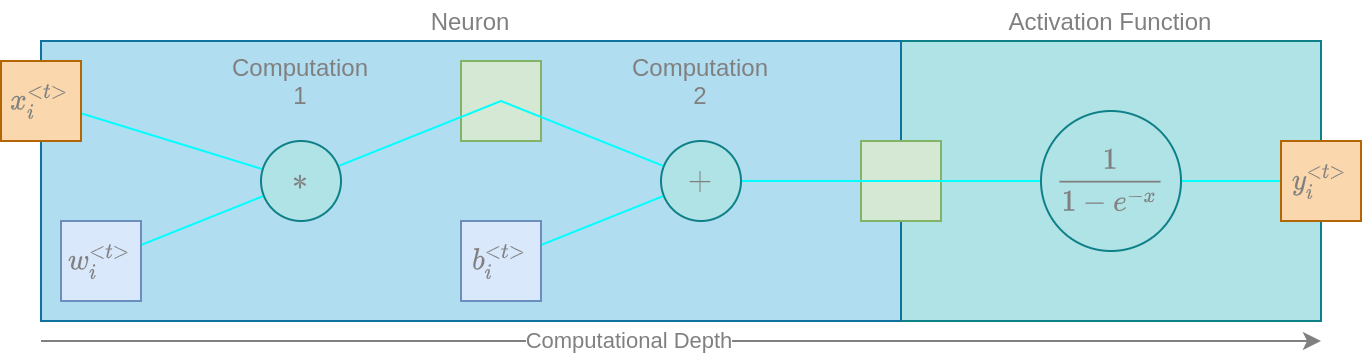
\includegraphics[width=1\linewidth]{neuron.png}
          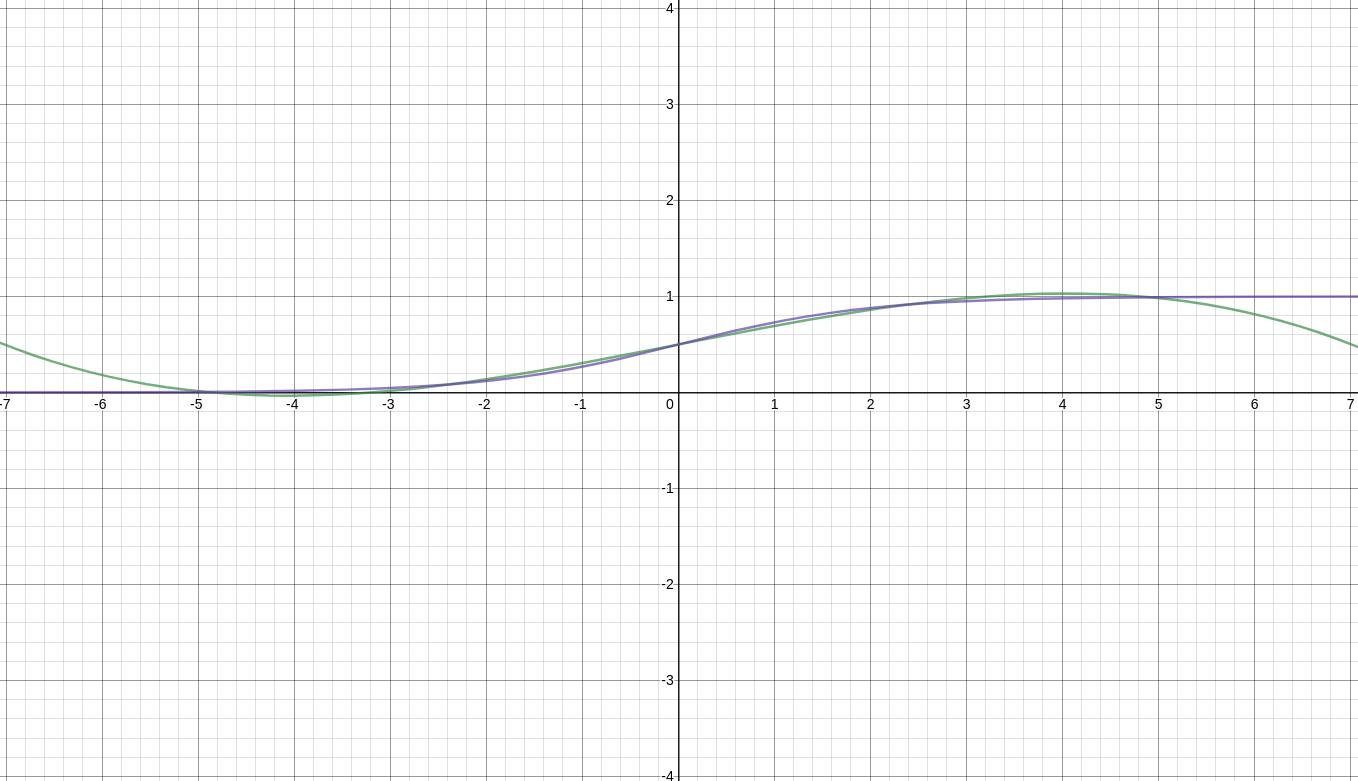
\includegraphics[width=1\linewidth]{desmos.png}
        \end{column}
        \begin{column}{0.5\textwidth}
          \begin{itemize}
            \item There is a problem though, that activation has a divide!
            \item Thats ok, lets approximate.
            \item Approximation works well as a polynomial between -5 and 5
          \end{itemize}
        \end{column}
      \end{columns}
    \end{frame}

    \begin{frame}{Deep Learning $+$ Fully Homomorphic Encryption}
      Example 1D convolutional neural network used in our pipeline with approximation \\
      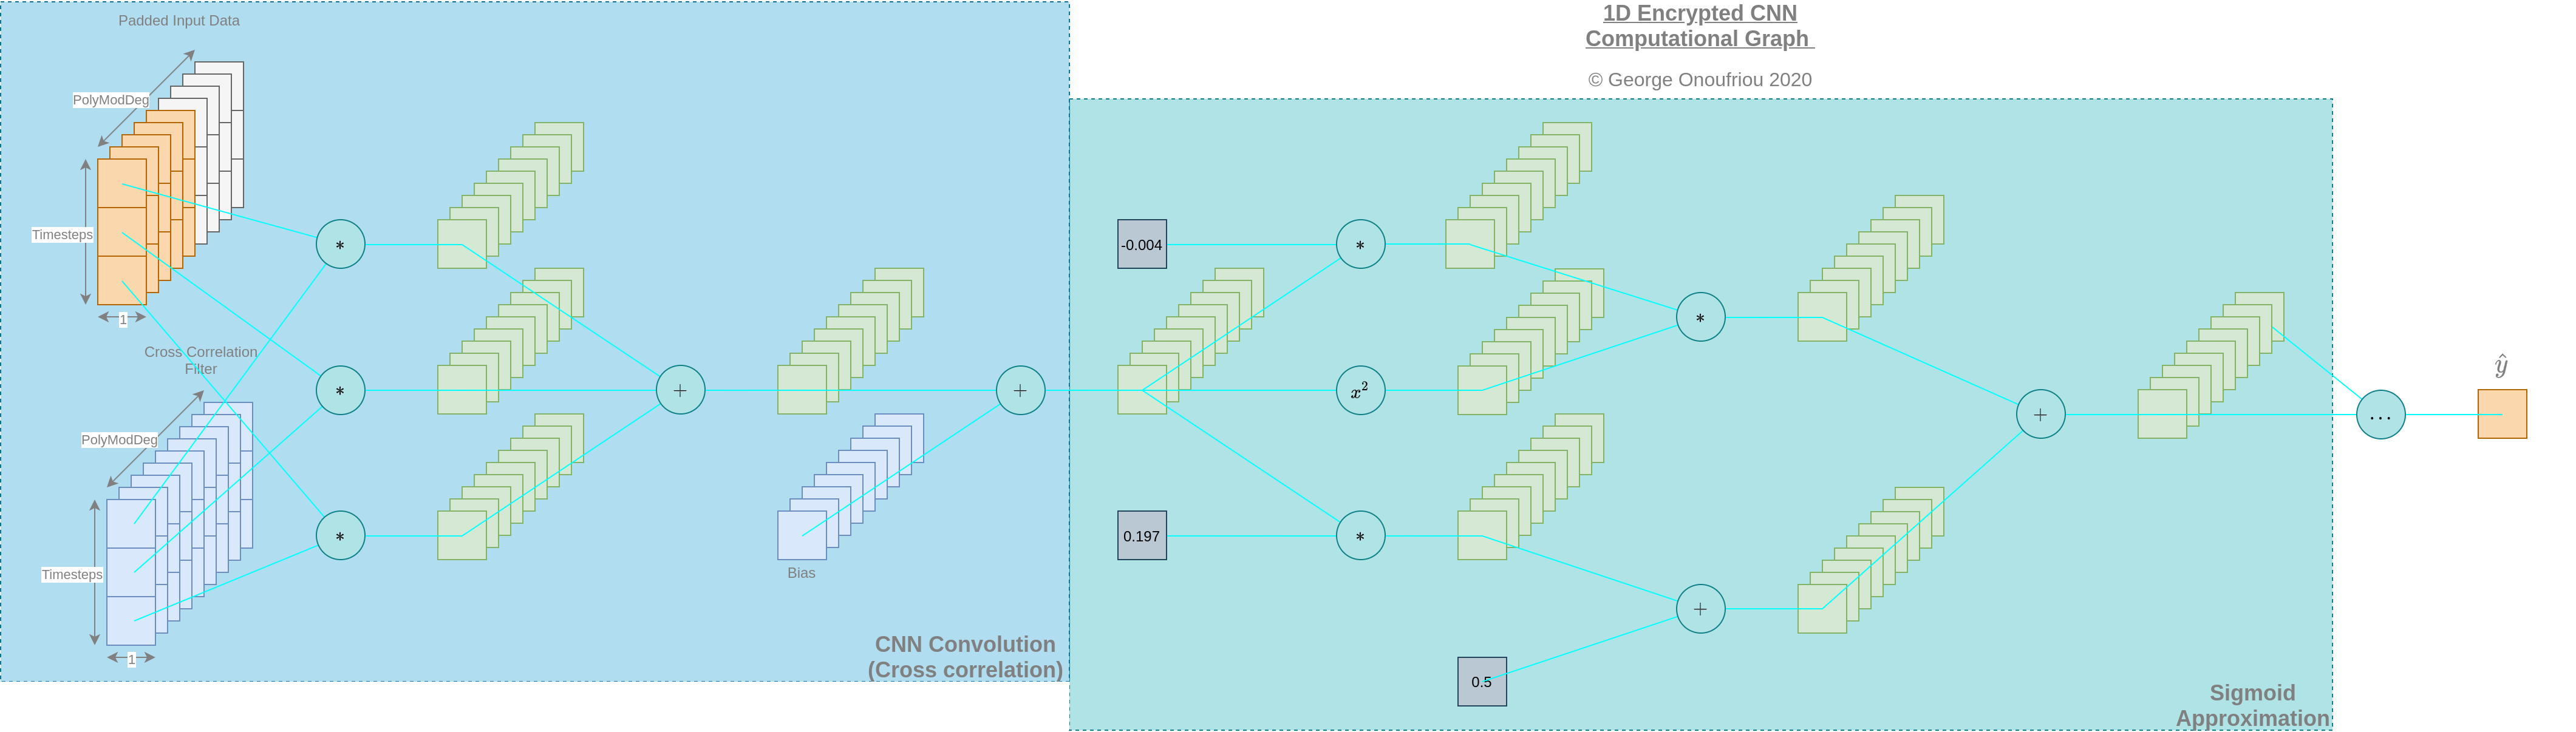
\includegraphics[width=1\linewidth]{encrypted_cnn.png}
    \end{frame}

    \begin{frame}{As a pipeline}
      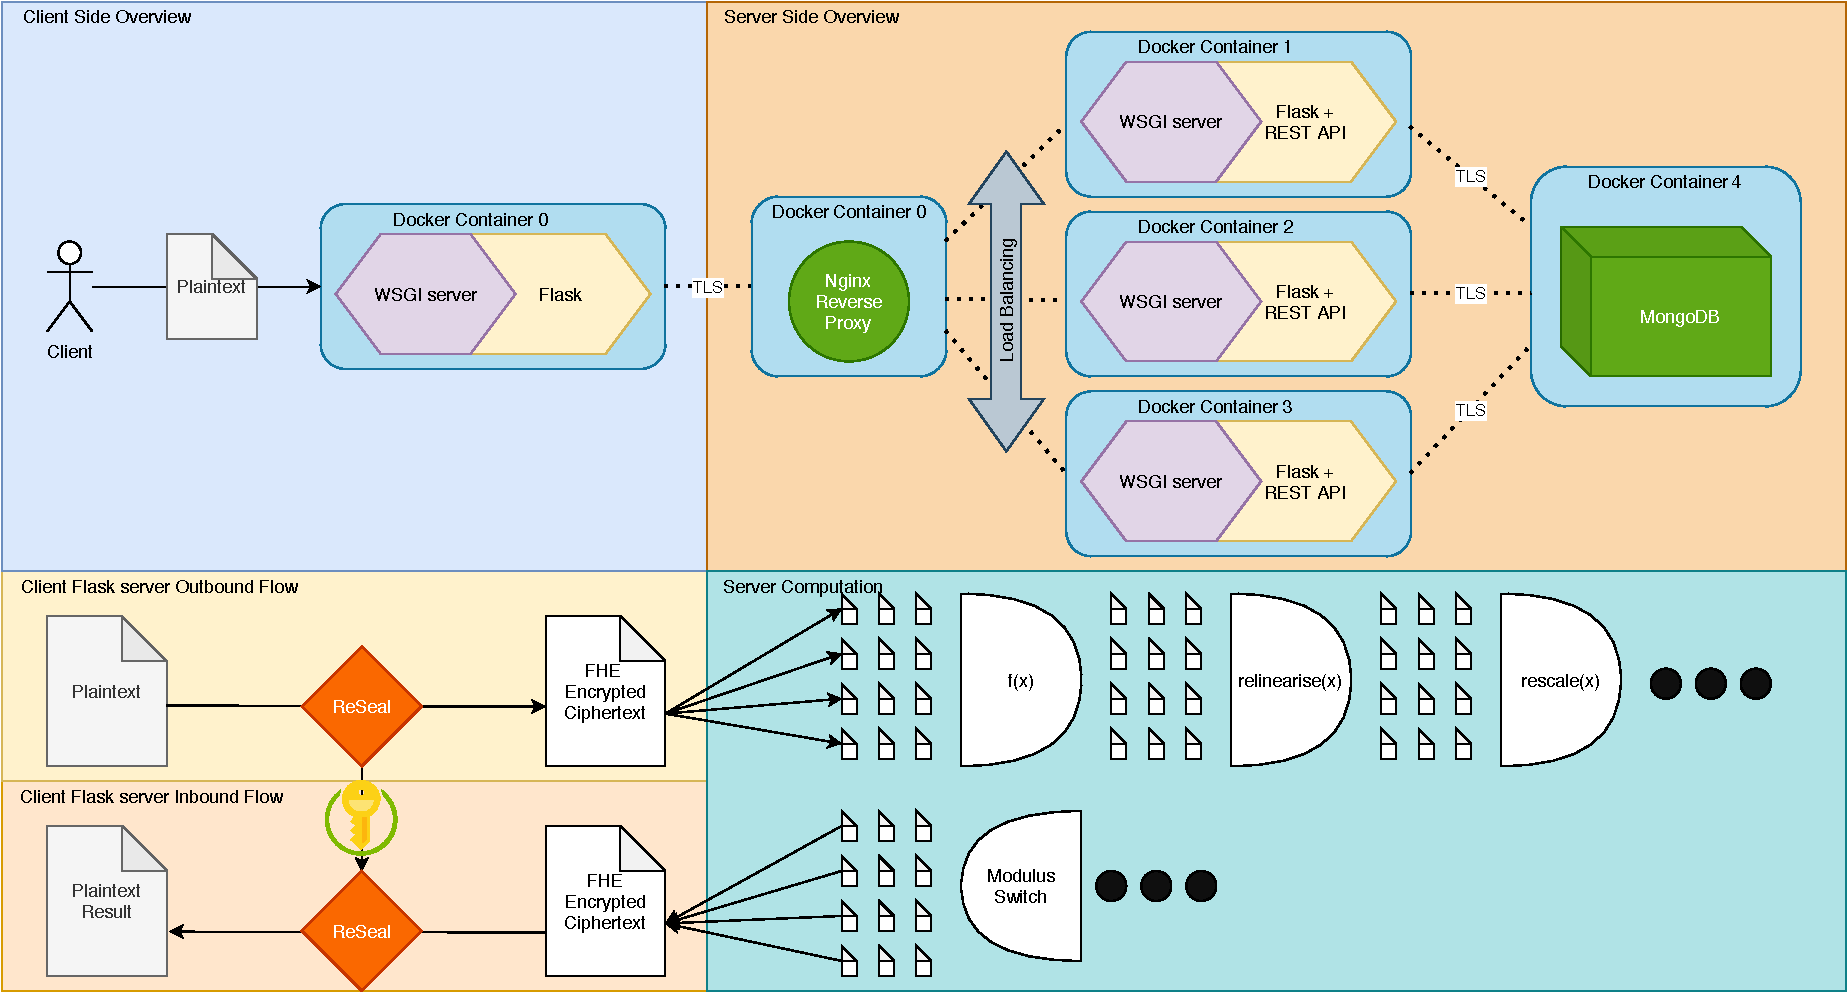
\includegraphics[width=0.85\linewidth]{nextgen.pdf}
    \end{frame}

  \section{Results}

    \begin{frame}{Computational Complexity}
      \begin{table}[]
        \begin{tabular}{l|ll}
        Operation               & \begin{tabular}[c]{@{}l@{}}Locally \\ (seconds 3.s.f)\end{tabular} & \begin{tabular}[c]{@{}l@{}}Remotely\\ (seconds 3.s.f)\end{tabular} \\ \hline
        Encryption              & $0.0136$                                                             & $0.454$                                                              \\
        Decryption              & $0.0330$*                                                            & $1.14$*                                                              \\
        Inference               & $0.966$** *                                                                   & $3.13$** *                                                           \\
        Ciphertext $+$ Ciphertext & $0.287$*                                                             & -                                                                  \\
        Ciphertext $+$ Plaintext  & $0.0480$*                                                            & -                                                                  \\
        Ciphertext $*$ Ciphertext & $0.277$*                                                             & -                                                                  \\
        Ciphertext $*$ Plaintext  & $0.0500$*                                                            & -
        \end{tabular}
      \end{table}
    \end{frame}

  \section{Future Direction}

    \begin{frame}{Future Plans}
      \begin{columns}
        \begin{column}{0.5\textwidth}
          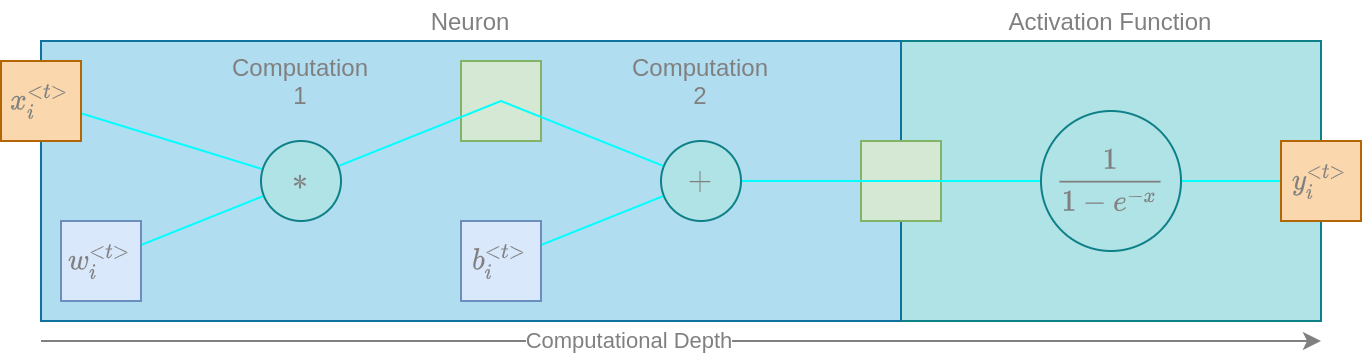
\includegraphics[width=1\linewidth]{neuron.png}
        \end{column}
        \begin{column}{0.5\textwidth}
          \begin{itemize}
            \item Improve on the pipeline; faster, wider, more variety in networks.
            \item Tackling the training problem; improve results using  transfer learning to minimize learning.
            \item Accelerate more computations onto GPU.
          \end{itemize}
        \end{column}
      \end{columns}
    \end{frame}

  \section{Summary}

    \begin{frame}{Conclusion}
      \begin{columns}
        \begin{column}{0.5\textwidth}
          \begin{itemize}
            \item Created open python FHE abstraction library.
            \item Library used to show computation of arbitrary polynomial functions.
            \item Created computational graphs for FHE applied to deep learning.
            \item Used our library as a component in a larger pipeline, and the time taken to operate within this pipeline.
            \item Created an online web app demo to show how it will work to non-technical level.
            \item Create an online web REST API for our pipeline itself to operate over the Internet securely.
          \end{itemize}
        \end{column}
      \end{columns}
    \end{frame}

  \section{Bibliography}

    \begin{frame}[allowframebreaks]
      \frametitle{References}
      \bibliographystyle{unsrt}
      \bibliography{./src/fhe.bib}%must have no space after ,
    \end{frame}

  \section{Appendix}

    % \begin{frame}[allowframebreaks]
    %   \frametitle{Appendix}
    % \end{frame}

    \begin{frame}{Acknowledgments}
      \begin{columns}
        \begin{column}{0.5\textwidth}
          \begin{itemize}
            \item This project received funding from the UKRI-EPSRC grant “The Internet of Food Things” (EP/R045127/1)
          \end{itemize}
        \end{column}
      \end{columns}
    \end{frame}


\end{document}
